
\documentclass[border=10pt, 12pt]{standalone}
\usepackage[svgnames]{xcolor}
\usepackage{amsmath}
\usepackage{pgfplots}
\pgfplotsset{compat=newest}
\usepackage[sfdefault]{FiraSans}
\usepackage{FiraMono}
\renewcommand*\familydefault{\sfdefault}
\begin{document}
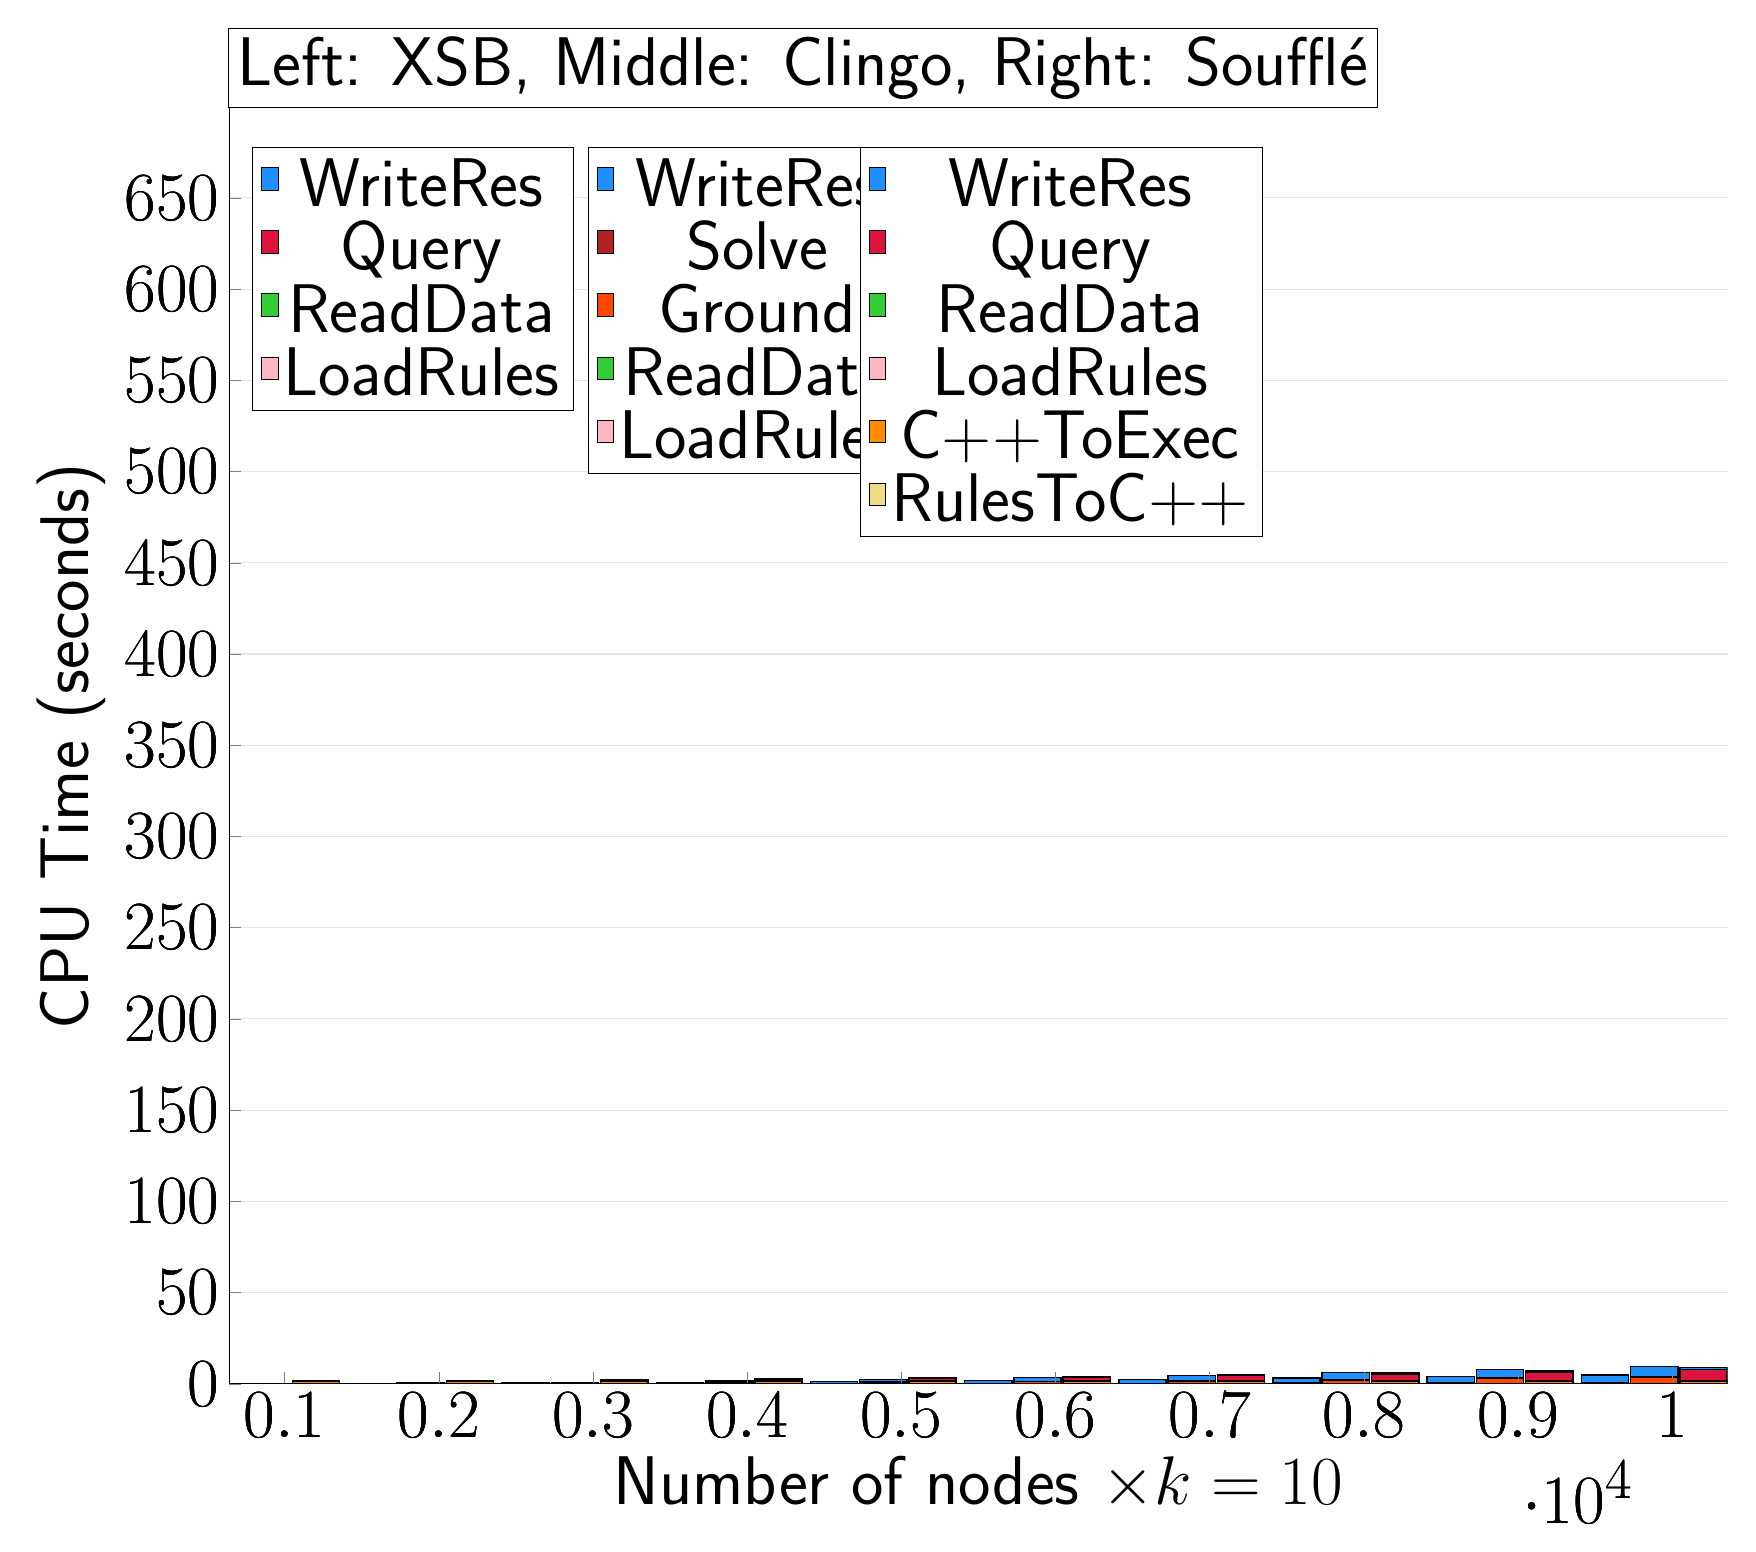
\begin{tikzpicture}
                        \begin{axis}[bar shift=-24.3pt, 
   ybar stacked,
   width=1.7\textwidth,
   bar width=0.6cm,
   ymajorgrids, tick align=inside,
   major grid style={draw=gray!20},
   xtick=data,
   ymin=0, ymax=699.059,
   axis x line*=bottom,
   axis y line*=left,
   enlarge x limits=0.04,
   legend style={
       at={(0.23, 0.97)},
       anchor=north east,
       legend columns=1,
       font=\Huge,
   },
   ylabel={CPU Time (seconds)},
   xlabel={Number of nodes $\times k=10$},
   label style={font=\Huge},
   tick label style={font=\Huge},
]
\addlegendimage{fill=DodgerBlue, draw=black, line width=0.2pt}
\addlegendentry{WriteRes}
\addlegendimage{fill=Crimson, draw=black, line width=0.2pt}
\addlegendentry{Query}
\addlegendimage{fill=LimeGreen, draw=black, line width=0.2pt}
\addlegendentry{ReadData}
\addlegendimage{fill=LightPink, draw=black, line width=0.2pt}
\addlegendentry{LoadRules}
\addplot +[fill=LightPink, draw=black, line width=0.55pt] coordinates {
(1000, 0.0005473999999999993)
(2000, 0.0005462000000000006)
(3000, 0.0005476000000000002)
(4000, 0.0005489999999999998)
(5000, 0.000547000000000001)
(6000, 0.0005456000000000005)
(7000, 0.0005539999999999996)
(8000, 0.0005478)
(9000, 0.0005606)
(10000, 0.0005481999999999997)
};
\addplot +[fill=LimeGreen, draw=black, line width=0.55pt] coordinates {
(1000, 0.0008912000000000006)
(2000, 0.0017154)
(3000, 0.0025437999999999997)
(4000, 0.0033607999999999997)
(5000, 0.00423)
(6000, 0.005051600000000001)
(7000, 0.005836399999999999)
(8000, 0.006659000000000001)
(9000, 0.007503999999999999)
(10000, 0.0083746)
};
\addplot +[fill=Crimson, draw=black, line width=0.55pt] coordinates {
(1000, 0.004786799999999999)
(2000, 0.0198008)
(3000, 0.0443262)
(4000, 0.08116300000000001)
(5000, 0.1321064)
(6000, 0.19463460000000002)
(7000, 0.27124139999999997)
(8000, 0.3612752)
(9000, 0.4486312)
(10000, 0.5769643999999999)
};
\addplot +[fill=DodgerBlue, draw=black, line width=0.55pt] coordinates {
(1000, 0.04190819999999999)
(2000, 0.1667948)
(3000, 0.376666)
(4000, 0.6669968)
(5000, 1.0454700000000001)
(6000, 1.5000931999999998)
(7000, 2.0344336)
(8000, 2.6812662)
(9000, 3.4351062)
(10000, 4.165259999999999)
};
\end{axis}

\begin{axis}[bar shift=-6.5pt, 
   ybar stacked,
   width=1.7\textwidth,
   bar width=0.6cm,
   ymajorgrids, tick align=inside,
   major grid style={draw=none},
   xtick=data,
   ymin=0, ymax=699.059,
   axis x line*=none,
   axis y line*=none,
   enlarge x limits=0.04,
   legend style={
       at={(0.454, 0.97)},
       anchor=north east,
       legend columns=1,
       font=\Huge,
   },
   label style={font=\Huge},
   tick label style={font=\Huge},
]
\addlegendimage{fill=DodgerBlue, draw=black, line width=0.2pt}
\addlegendentry{WriteRes}
\addlegendimage{fill=FireBrick, draw=black, line width=0.2pt}
\addlegendentry{Solve}
\addlegendimage{fill=OrangeRed, draw=black, line width=0.2pt}
\addlegendentry{Ground}
\addlegendimage{fill=LimeGreen, draw=black, line width=0.2pt}
\addlegendentry{ReadData}
\addlegendimage{fill=LightPink, draw=black, line width=0.2pt}
\addlegendentry{LoadRules}
\addplot +[fill=LightPink, draw=black, line width=0.55pt] coordinates {
(1000, 0.0)
(2000, 0.0)
(3000, 0.0)
(4000, 0.0)
(5000, 0.0)
(6000, 0.0)
(7000, 0.0)
(8000, 0.0)
(9000, 0.0)
(10000, 0.0)
};
\addplot +[fill=LimeGreen, draw=black, line width=0.55pt] coordinates {
(1000, 0.0)
(2000, 0.0)
(3000, 0.0)
(4000, 0.006000000000000005)
(5000, 0.010000000000000009)
(6000, 0.010000000000000009)
(7000, 0.010000000000000009)
(8000, 0.01200000000000001)
(9000, 0.020000000000000018)
(10000, 0.020000000000000018)
};
\addplot +[fill=OrangeRed, draw=black, line width=0.55pt] coordinates {
(1000, 0.030000000000000027)
(2000, 0.118)
(3000, 0.268)
(4000, 0.48200000000000004)
(5000, 0.79)
(6000, 1.18)
(7000, 1.6179999999999999)
(8000, 2.1300000000000003)
(9000, 2.806)
(10000, 3.4299999999999997)
};
\addplot +[fill=FireBrick, draw=black, line width=0.55pt] coordinates {
(1000, 0.0)
(2000, 0.010000000000000009)
(3000, 0.02400000000000002)
(4000, 0.052000000000000046)
(5000, 0.08200000000000006)
(6000, 0.1260000000000001)
(7000, 0.16599999999999993)
(8000, 0.21399999999999988)
(9000, 0.27000000000000013)
(10000, 0.3540000000000002)
};
\addplot +[fill=DodgerBlue, draw=black, line width=0.55pt] coordinates {
(1000, 0.06)
(2000, 0.23199999999999993)
(3000, 0.526)
(4000, 0.9279999999999999)
(5000, 1.448)
(6000, 2.06)
(7000, 2.8760000000000003)
(8000, 3.716)
(9000, 4.637999999999999)
(10000, 5.746)
};
\end{axis}

\begin{axis}[bar shift=11.3pt, 
   ybar stacked,
   width=1.7\textwidth,
   bar width=0.6cm,
   ymajorgrids, tick align=inside,
   major grid style={draw=none},
   xtick=data,
   ymin=0, ymax=699.059,
   axis x line*=none,
   axis y line*=none,
   enlarge x limits=0.04,
   legend style={
       at={(0.69, 0.97)},
       anchor=north east,
       legend columns=1,
       font=\Huge,
   },
   label style={font=\Huge},
   tick label style={font=\Huge},
]
\addlegendimage{fill=DodgerBlue, draw=black, line width=0.2pt}
\addlegendentry{WriteRes}
\addlegendimage{fill=Crimson, draw=black, line width=0.2pt}
\addlegendentry{Query}
\addlegendimage{fill=LimeGreen, draw=black, line width=0.2pt}
\addlegendentry{ReadData}
\addlegendimage{fill=LightPink, draw=black, line width=0.2pt}
\addlegendentry{LoadRules}
\addlegendimage{fill=DarkOrange, draw=black, line width=0.2pt}
\addlegendentry{C++ToExec}
\addlegendimage{fill=LightGoldenrod, draw=black, line width=0.2pt}
\addlegendentry{RulesToC++}
\addplot +[fill=LightGoldenrod, draw=black, line width=0.55pt] coordinates {
(1000, 0.0020000000000000005)
(2000, 0.004000000000000001)
(3000, 0.006000000000000001)
(4000, 0.0020000000000000005)
(5000, 0.0020000000000000005)
(6000, 0.006000000000000001)
(7000, 0.006000000000000001)
(8000, 0.0020000000000000005)
(9000, 0.0020000000000000005)
(10000, 0.0020000000000000005)
};
\addplot +[fill=DarkOrange, draw=black, line width=0.55pt] coordinates {
(1000, 1.4659999999999997)
(2000, 1.472)
(3000, 1.47)
(4000, 1.4700000000000002)
(5000, 1.472)
(6000, 1.472)
(7000, 1.474)
(8000, 1.4780000000000002)
(9000, 1.4740000000000002)
(10000, 1.4600000000000002)
};
\addplot +[fill=LightPink, draw=black, line width=0.55pt] coordinates {
(1000, 0.0001648)
(2000, 0.00016160000000000002)
(3000, 0.0001718)
(4000, 0.00017460000000000002)
(5000, 0.00017839999999999997)
(6000, 0.00016879999999999998)
(7000, 0.0001764)
(8000, 0.00015560000000000001)
(9000, 0.00017859999999999998)
(10000, 0.0001346)
};
\addplot +[fill=LimeGreen, draw=black, line width=0.55pt] coordinates {
(1000, 0.0040606)
(2000, 0.007179200000000001)
(3000, 0.010138999999999999)
(4000, 0.013042199999999999)
(5000, 0.0144368)
(6000, 0.0176474)
(7000, 0.0197192)
(8000, 0.0186252)
(9000, 0.0236118)
(10000, 0.021443999999999998)
};
\addplot +[fill=Crimson, draw=black, line width=0.55pt] coordinates {
(1000, 0.0705446)
(2000, 0.230699)
(3000, 0.5187272)
(4000, 0.9394866000000001)
(5000, 1.486266)
(6000, 2.15974)
(7000, 2.9822819999999997)
(8000, 3.9257280000000003)
(9000, 5.0209600000000005)
(10000, 6.306964)
};
\addplot +[fill=DodgerBlue, draw=black, line width=0.55pt] coordinates {
(1000, 0.010958199999999998)
(2000, 0.0433486)
(3000, 0.0969962)
(4000, 0.17452120000000002)
(5000, 0.2696992)
(6000, 0.3851424)
(7000, 0.525613)
(8000, 0.7083472)
(9000, 0.866398)
(10000, 1.079556)
};
\end{axis}


\node[anchor=south, draw, fill=white] at (rel axis cs:0.42,1) {\Huge Left: XSB, Middle: Clingo, Right: Soufflé};
\end{tikzpicture}
\end{document}
                    